\documentclass[UTF8,12pt,a4paper]{ctexart}
\usepackage{amsmath,amssymb,bm,booktabs,graphicx,geometry,float,hyperref}
\geometry{left=2.3cm,right=2.3cm,top=2.5cm,bottom=2.5cm}
\title{基于SVD的七关节闭链机构奇异性分析}
\author{}
\date{\today}
\begin{document}
\maketitle
\tableofcontents

\section{SVD方法简介}
对任意矩阵$A\in\mathbb R^{m\times n}$，奇异值分解写为
\[
A=U\Sigma V^{\mathsf T},
\]
其中$U$与$V$为正交矩阵，$\Sigma$的对角元满足
\[
\sigma_1\ge\sigma_2\ge\cdots\ge\sigma_r\ge0.
\]
最小奇异值刻画矩阵距离秩亏的程度。当$\sigma_{\min}=0$时矩阵不满秩；
当其接近零时，速度映射病态，机构接近奇异构型。

\section{完整闭环速度方程}
纯编号替换后的链位置标签依次为$(2,3,4,5,6,7,1)$。第$j$个转动关节
对闭环末端速度的Jacobian列为
\[
J_j=
\begin{bmatrix}
\bm z_j\times(\bm p_e-\bm p_j)\\
\bm z_j
\end{bmatrix}.
\]
完整闭环速度约束为$J\dot{\bm q}=0$。以新$q_2$为驱动关节，将其列记为
$J_a$，其余六列组成
\[
J_p=
\left[J_{q_3}\;J_{q_4}\;J_{q_5}\;J_{q_6}\;J_{q_7}\;J_{q_1}\right]
\in\mathbb R^{6\times6}.
\]
因此
\[
J_p\dot{\bm q}_p=-J_a\dot q_2.
\]
当$\det(J_p)=0$或$\sigma_6(J_p)=0$时，被动速度不能由给定$\dot q_2$
唯一确定，完整七关节闭链机构处于奇异构型。

\section{当前$s=+1$分支的SVD结果}
\begin{figure}[H]
\centering
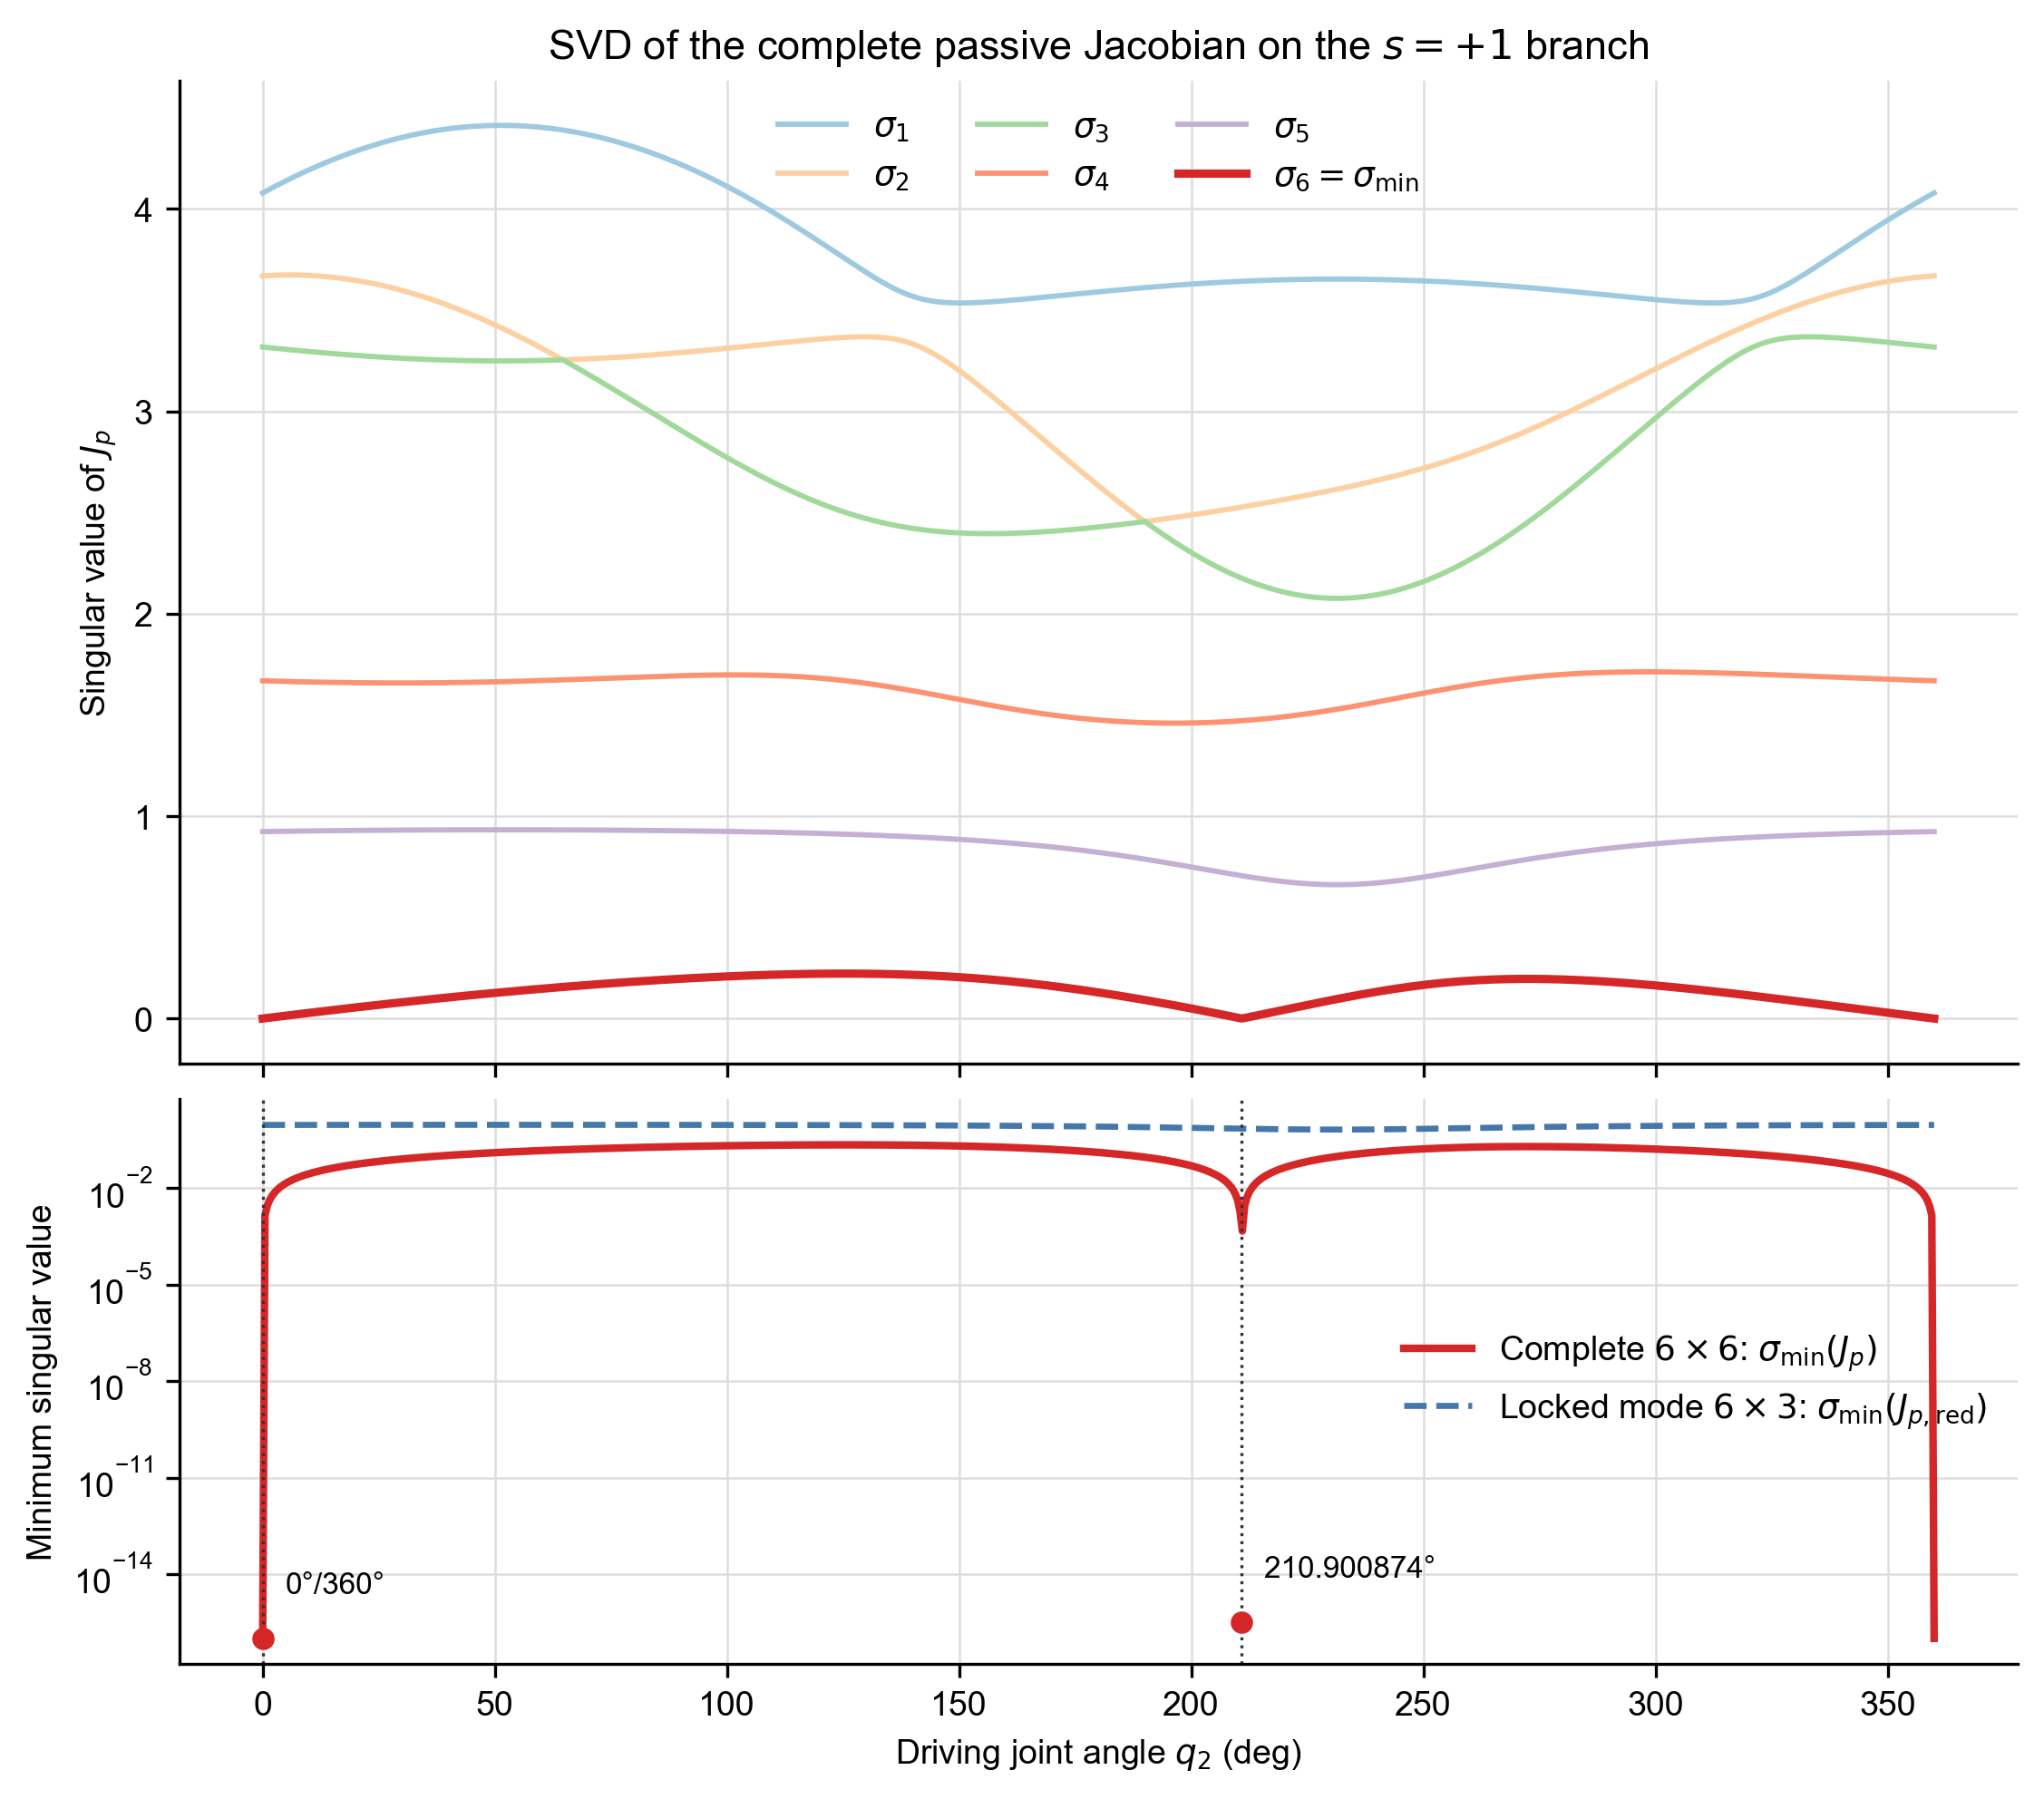
\includegraphics[width=0.94\textwidth]{singular_values.png}
\caption{完整被动Jacobian的六个奇异值及最小奇异值判据。}
\end{figure}

对$q_2\in[0,360^\circ]$扫描，并对行列式变号区间使用Brent法精确求根。
\begin{table}[H]
\centering
\caption{完整被动Jacobian的奇异位置}
\begin{tabular}{rrrrrr}
\toprule
$q_2$ (deg) & $q_1$ (deg) & $q_4$ (deg) & $q_6$ (deg)
& $\sigma_{\min}(J_p)$ & rank\\
\midrule
0/360 & 0.000000 & 0.000000 & 0.000000 & 5.000e-17 & 5 \\
210.900874173 & -149.099126 & 30.900874 & -30.900874 & 3.196e-16 & 5 \\
\bottomrule
\end{tabular}
\end{table}
$0^\circ$与$360^\circ$是同一个周期构型，只计作一个独立奇异位置。
内部奇异位置为
\[
q_2=210.900874173^\circ.
\]

\section{锁定后约化Jacobian}
指定平面模式中$q_3,q_5,q_7$锁死。仅保留$q_4,q_6,q_1$时，
\[
J_{p,\mathrm{red}}=
\left[J_{q_4}\;J_{q_6}\;J_{q_1}\right]
\in\mathbb R^{6\times3}.
\]
其整周最小奇异值为0.661314604，出现在
$q_2\approx231.500^\circ$，始终大于零。该结果说明锁定后的
平面四杆速度映射保持满列秩，但不能替代完整七关节机构的奇异性判定。

\section{结论}
\begin{enumerate}
\item 完整$6\times6$被动Jacobian是七关节机构奇异性分析的主判据。
\item 当前$s=+1$分支的独立奇异构型位于$0^\circ/360^\circ$和
$210.900874173^\circ$。
\item 稀疏采样可能只能得到约$0.0015$的最小值；精确求根后
$\sigma_{\min}$处于$10^{-16}$数值量级。
\item $6\times3$约化矩阵整周满列秩，只说明锁定后的指定运动模式不退化。
\end{enumerate}
\end{document}
